\documentclass[10pt,a4paper,notitlepage]{report}
\usepackage[utf8]{inputenc}
\usepackage{amsmath}
\usepackage{amsfonts}
\usepackage{amssymb}
\usepackage{hyperref}
\usepackage[margin=1in]{geometry}
\usepackage{fancyhdr}
\usepackage[svgnames]{xcolor}
\usepackage{graphicx}
\usepackage{minted}

\usemintedstyle{manni}
\pagestyle{fancy}
\fancyhead[L]{\small Decoding Neuronal EEG Activity}
\fancyhead[R]{\small\textsc{Problem 2}}
\renewcommand{\headrulewidth}{0.4pt}
\fancyfoot[C]{\thepage}

%\newcommand{\code}[1]{\colorbox{lightgray}{\texttt{#1}}}

\begin{document}

\paragraph*{GENERAL REMARKS} The programming problems require you to fill the gaps in the provided MATLAB scripts. Use the problem description below and the comments in the code to solve the problems. The missing parts are typically indicated by '\texttt{...}' (not to be confused with line breaks!), where each '\texttt{...}' might be replaced by multiple lines of code. Following the provided code is recommended but only leads you to one of many possible solutions. If some part of the code seems unclear or counterintuitive to you, feel free to depart from it. Be aware, however, that the suggested variable names and structures are typically used later in the script, e.g. for plotting, and occur again in other scripts and problems. In any case, your code should produce the same output as the Musterlösung. \textbf{Note}: To be able to run the code, you must have the Statistics, Signal Processing, Image Processing, and Wavelet toolboxes installed, and you must have the folder \texttt{utility} and all subfolders as well as the location of the ECG/EEG datasets added to your MATLAB path.

\section*{Problem 2}
In this problem, we want to look at electrocartiographic (ECG) data from a pig under different levels of blood dilution (see Scheller et al., 2011). We will pre-process the data from one ECG channel over 8 experimental blocks, examine the data closely, extract some meaningful features, and perform classification of two arbitrary blocks, using support vector machines (SVMs) in addition to logistic regression. The scripts \texttt{runECG<1,2,3>.m} will successively build the final program, together with the slightly modified classification function \texttt{modelFitVal2.m}. MATLAB's \texttt{fdatool} will be used to build the necessary filters.

\section*{Part 1: Basic Processing, Understanding ECG}
In \texttt{runECG1.m} we will examine a short example signal covering 1 minute of ECG. First, the sampling rate and corresponding period are defined and channel 3 of the example dataset is loaded. Also, a high-pass and a low-pass filter are loaded, which assumes that those filters exist. 

\begin{minted}[xleftmargin=1cm]{matlab}
srate = 512;
T = 1/srate;

load('ECG_signal_3')
signal = ECG_signal(:, 3);

load('filterHP_0.5_1.5.mat')
load('filterLP_3_10.mat')
\end{minted}

Use the command \texttt{fdatool} to construct a high-pass FIR filter with transition band edges at 0.5 Hz and 1.5 Hz, and a low-pass FIR filter with transition band edges at 3 Hz and 10 Hz. An FIR filter can be represented solely by a vector of coefficients (aka its numerator). Store each coefficient vector in the variables \texttt{filterHP} and \texttt{filterLP} under the \texttt{.mat} files specified in the code. Consult the course slides and MATLAB's documentation for technical questions about filter design.

We now use the filters to create a high-pass filtered and a band-pass filtered signal.

\begin{minted}[xleftmargin=1cm]{matlab}
signalHP = ...
signalBP = ...
\end{minted}

Find a way to avoid phase-shifting of the signals due to filtering.

Next, we extract the locations of the amplitude peaks of the QRS complexes using the high-pass filtered signal and, after that, compute the frequency power spectra for all three signals.

\begin{minted}[xleftmargin=1cm]{matlab}
[H2, HDR, s] = qrsdetect(signalHP, srate, 1);
peakPos = H2.EVENT.POS;

[spectrumFull, f_axis] = Powerspektrum(signal, T, 2048);
[spectrumHP, ~] = Powerspektrum(signalHP, T, 2048);
[spectrumBP, ~] = Powerspektrum(signalBP, T, 2048);
\end{minted}

Now we want to extract the phase for all signals. This means computing the analytic signal
\begin{equation*}
s_a(t)=s(t)+is_H(t)
\end{equation*}
where $s_H(t)$ is the Hilbert transform of $s(t)$, and obtaining its angle in radians in complex space.

\begin{minted}[xleftmargin=1cm]{matlab}
anaSignal = ...
anaSignalHP = ...
anaSignalBP = ...
phase = ...
phaseHP = ...
phaseBP = ...
\end{minted}

The phase angle is another time series of the same length as the signal. Find the appropriate functions and make sure you use them in the right way.

Next, we epoch the ECG signal, i.e. we rearrange the time series (we use only the high-pass filtered signal) into single heartbeats. First, we define a time window relative to the QRS peak location such that it covers the entire QRS complex including P and T wave.

\begin{minted}[xleftmargin=1cm]{matlab}
timeWindow = ...
\end{minted}

You might also want to include the following P wave, in order to examine the distance between heartbeats. You don't have to worry about overlaps or gaps between epochs – we just want each epoch to contain roughly one full QRS complex. Try to infer a reasonable time window from Scheller et al., 2011, and convert it to sample points.

Now we iterate over all QRS peaks, omitting the first and last peak to make sure our time window doesn't reach over the beginning or end of the signal. At each iteration, we select the signal within the current time window and subtract from it its mean.

\begin{minted}[xleftmargin=1cm]{matlab}
waves = nan(length(timeWindow), length(peakPos)-2);
for iEpoch=2:(length(peakPos)-1)
    wavesTmp = signalHP(...);
    waves(:, iEpoch-1) = wavesTmp - mean(wavesTmp);
end
\end{minted}

The next section of code produced plots, but a few lines must be edited near the end of the section. In order to plot all 8 channels contained in the dataset, we repeat the filtering and epoching part for all channels in a row. Complete the code by reproducing what you did before. We'll just reuse the QRS peak positions and time window from above.

\begin{minted}[xleftmargin=1cm]{matlab}
signalHP = ... 
waves = nan(length(timeWindow), length(peakPos)-2);
for iEpoch=2:(length(peakPos)-1)
    wavesTmp = signalHP(...);
    waves(:, iEpoch-1) = wavesTmp - mean(wavesTmp);
end
\end{minted}

\texttt{runECG1.m} is finished. It should produce the 6 figures below. The first 3 figures display the differences between the original, high-pass, and band-pass filtered signals, the last 3 figures characterize the QRS complex along the high-pass filtered signal. Try to understand what each plot tells you about the data.

\vspace{1cm}
\hspace{-1cm} 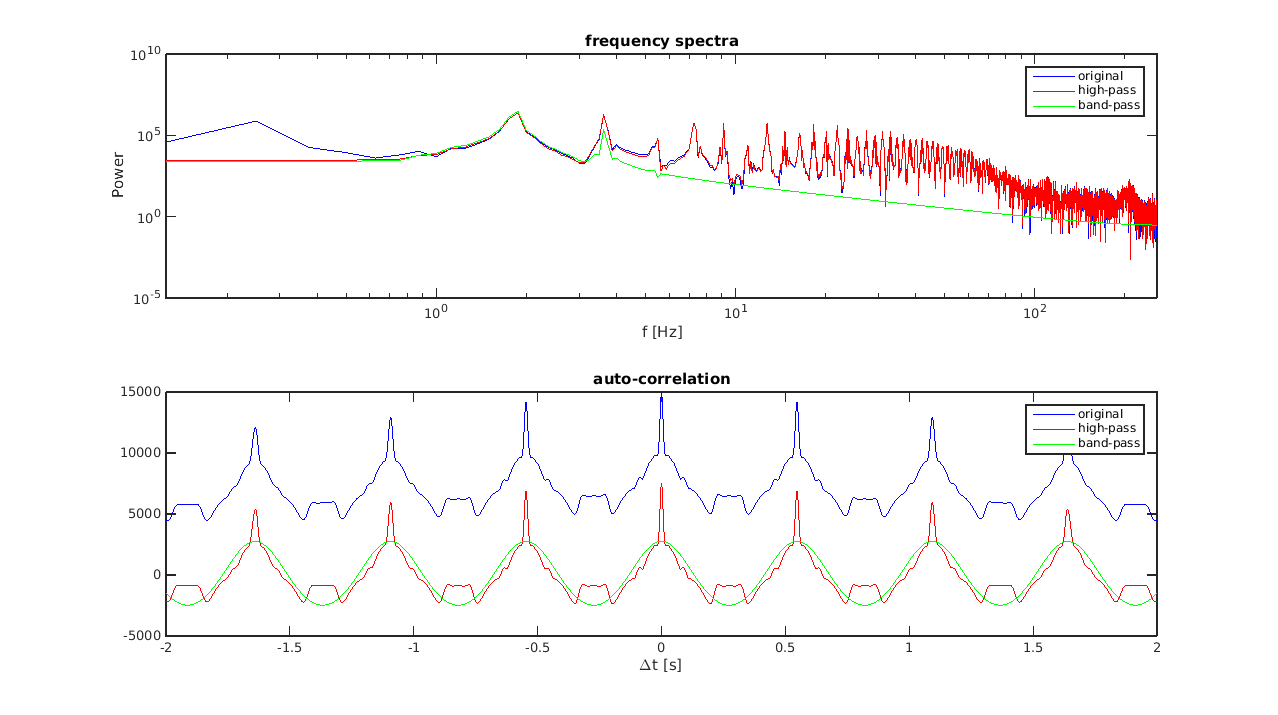
\includegraphics[scale=0.25]{p2fig1.png}
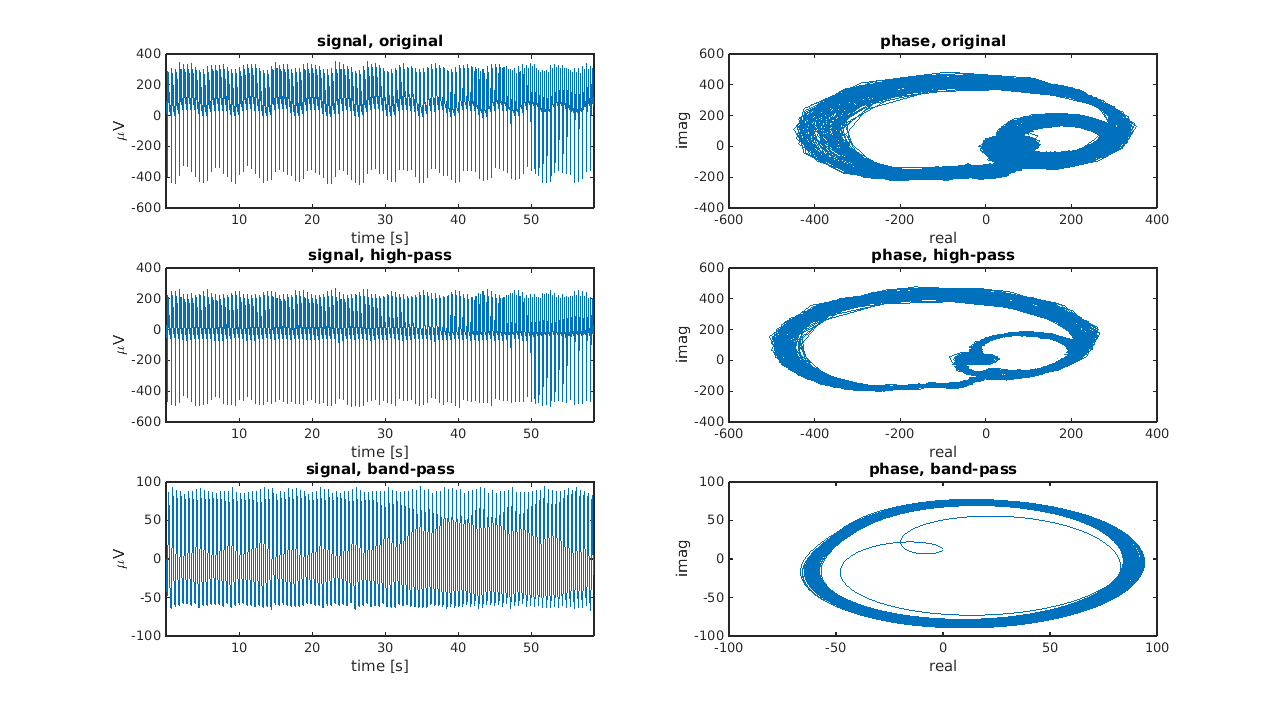
\includegraphics[scale=0.25]{p2fig2.png}

\hspace{-1cm} 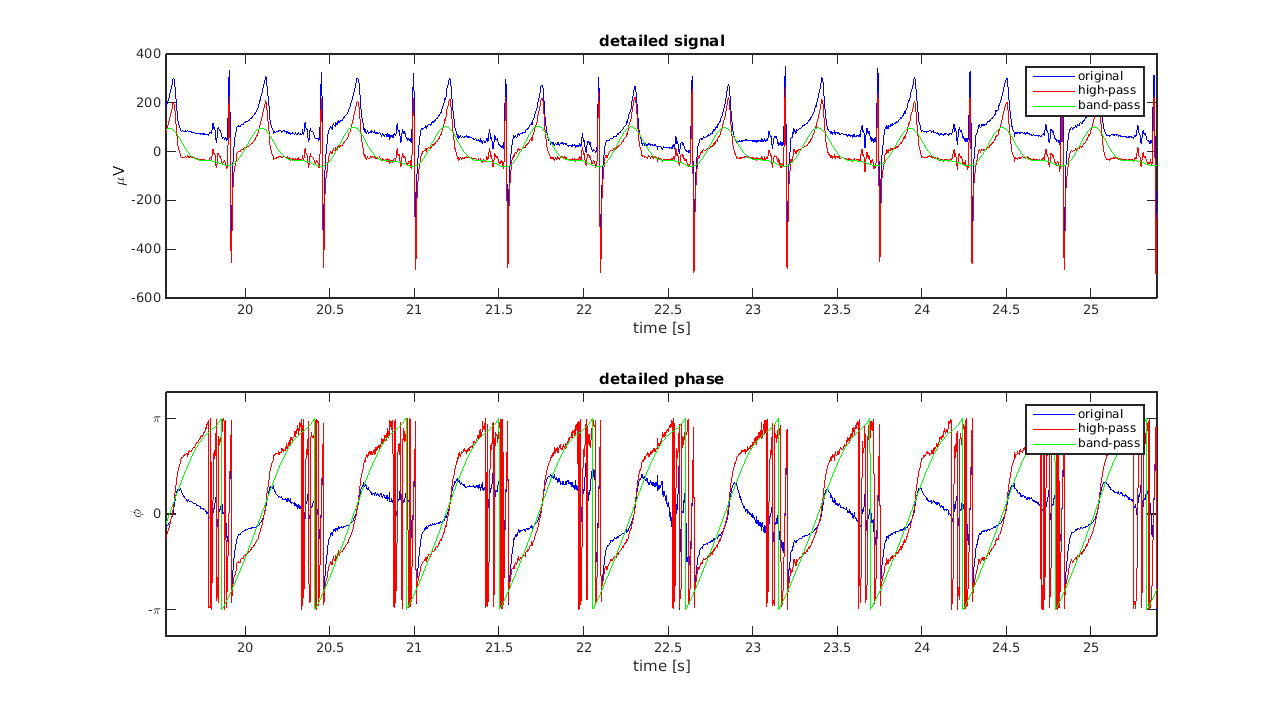
\includegraphics[scale=0.25]{p2fig3.png}
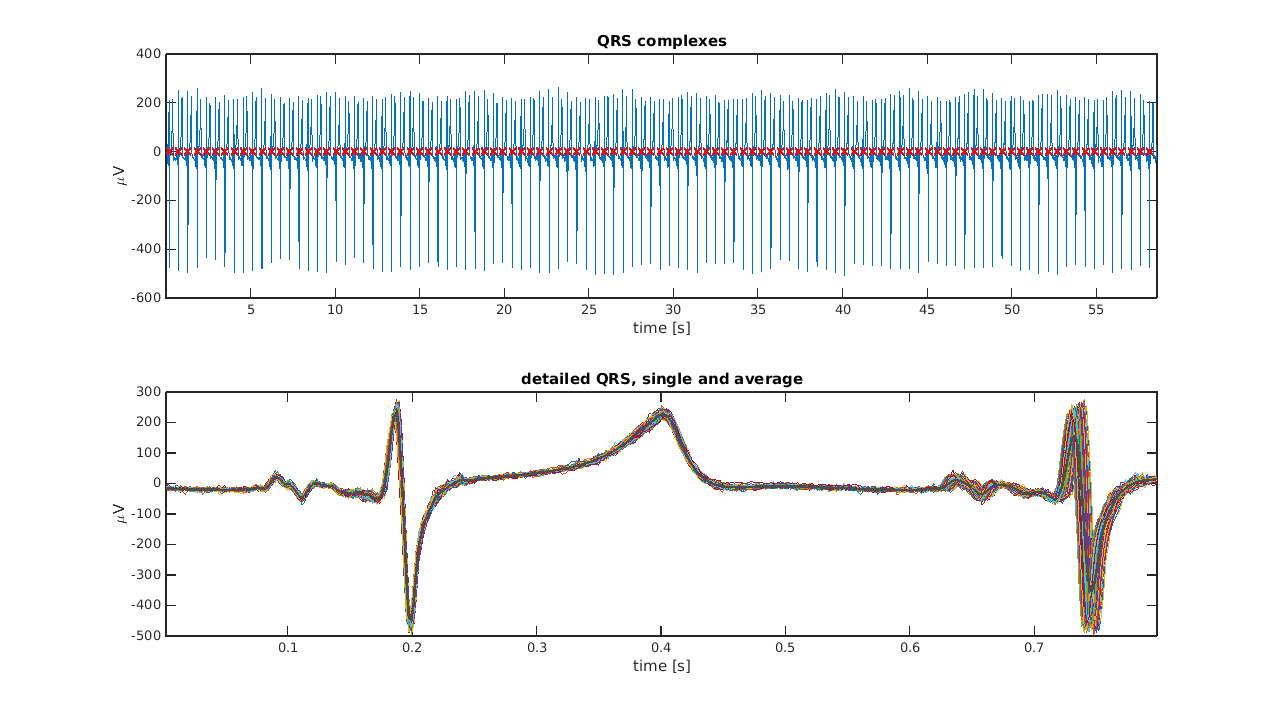
\includegraphics[scale=0.25]{p2fig4.png}

\hspace{-1cm} 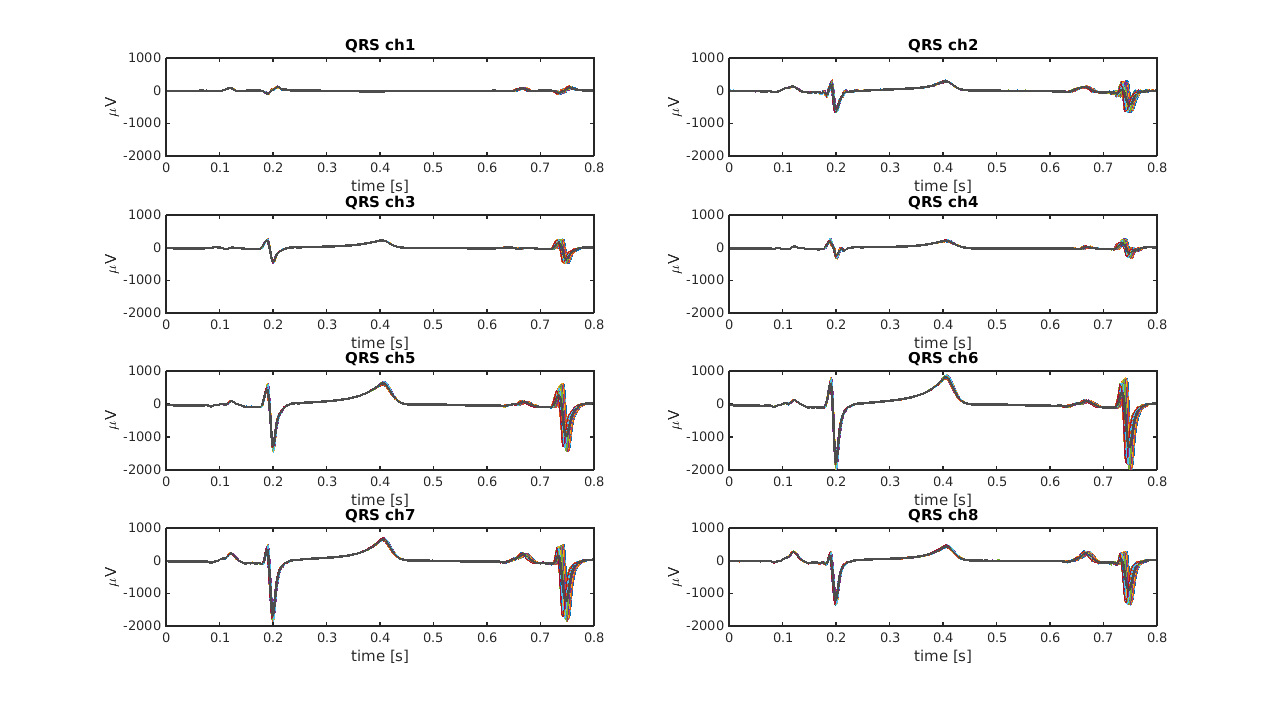
\includegraphics[scale=0.25]{p2fig5.png}
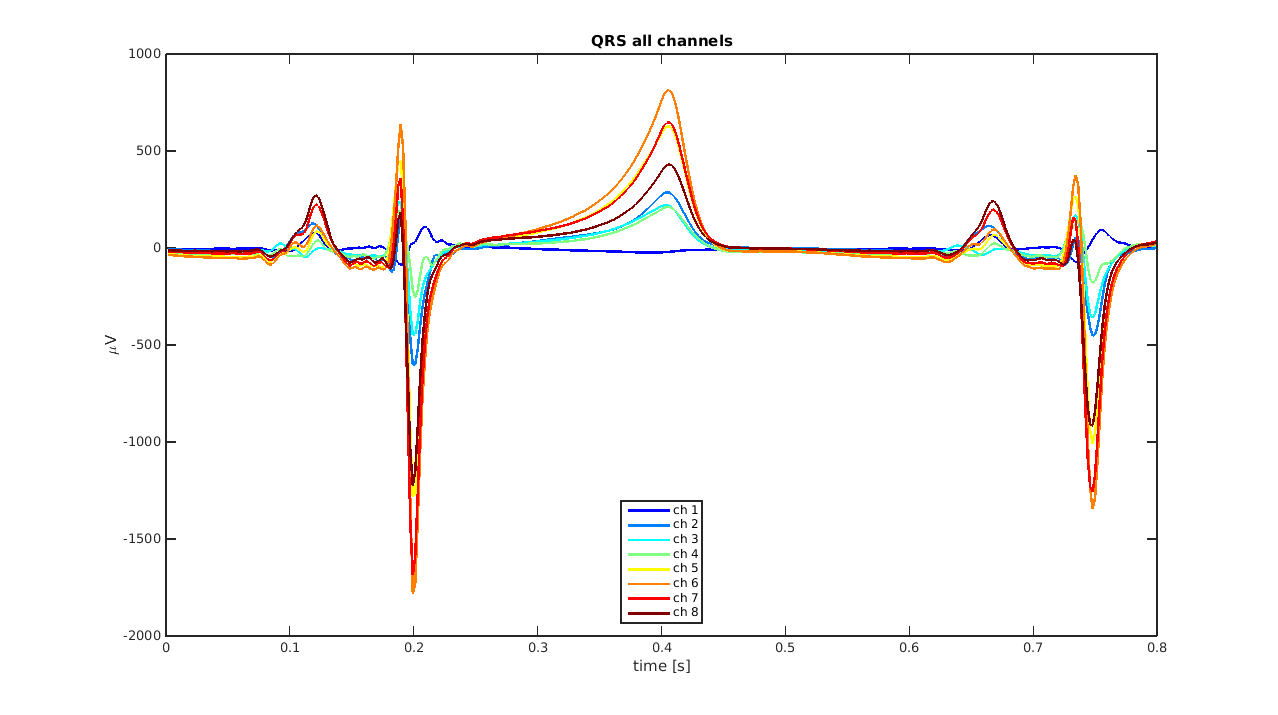
\includegraphics[scale=0.25]{p2fig6.png}


\section*{Part 2: Examining Features, Phase Locking}
\texttt{runECG2.m} builds on top of the previous script. We will now look at actual experimental data over 8 blocks of approx. 10 minutes each, recorded at increasing levels of blood dilution. We will only process channel 3 of the data.

We specify the sample frequency, load the same filters as before, initialize some figures, and set the pack size for later computing phase locking values. Then we start iterating over blocks and process each channel 3 signal analogous to the example signal before.

\begin{minted}[xleftmargin=1cm]{matlab}
srate = 512;

load('filterHP_0.5_1.5.mat')
load('filterLP_3_10.mat')

f1 = figure('units', 'normalized', 'outerposition', [0 0 1 1]);
f2 = figure('units', 'normalized', 'outerposition', [0 0 1 1]);
f3 = figure('units', 'normalized', 'outerposition', [0 0 1 1]);
f4 = figure('units', 'normalized', 'outerposition', [0 0 1 1]);

packSize = 11;

for B=1:8
\end{minted}

First, we load the signal, filter it, extract QRS peaks, and compute phases. Write the missing code for filtering and computing phases as before. We're only interested in the filtered signals, here.

\begin{minted}[xleftmargin=1cm]{matlab}
load(['block_' num2str(B)])
signal = block_data(:, 3);

signalHP = ...
signalBP = ...

[H2, HDR, s] = qrsdetect(signalHP, srate, 1);
peakPos = H2.EVENT.POS;

phaseHP = ...
phaseBP = ...
\end{minted}

Next, we epoch the high-pass filtered data. In addition to the ECG signal, we also epoch its phase.

\begin{minted}[xleftmargin=1cm]{matlab}
timeWindow = ...
waves = nan(length(timeWindow), length(peakPos)-2);
phases = nan(length(timeWindow), length(peakPos)-2);
for iEpoch=2:(length(peakPos)-1)
    wavesTmp = singalHP(...);
    waves(:, iEpoch-1) = wavesTmp - mean(wavesTmp);
    phasesTmp = unwrap(...);
    phases(:, iEpoch-1) = phasesTmp - ...
end
\end{minted}

We use the \texttt{unwrap} function to fold the sawtooth-shaped phase out of the interval $[-\pi, \pi]$ and shift each phase epoch up/down so it crosses zero at the QRS peak position. This way we make phase progression comparable among epochs. \texttt{waves} and \texttt{phases} will be of the same size, containing one epoch per column.

Based on the epoched phase, we can now compute the phase locking among consecutive epochs at each time point, using a sliding-window approach. We compute the phase locking value (PLV) at time $t$ over all epochs $k$ in pack $P$
\begin{equation*}
PLV_P(t) = \lvert \frac{1}{N}\sum_{k\in P}e^{i\phi_k(t)} \rvert
\end{equation*}
which is obtained by averaging the normalized complex phase over epochs and then taking the absolute value, which gives the magnitude of phase angle similarity within pack $P$. We define each pack as the $m$-neighborhood of each epoch $j$, including $j$:
\begin{equation*}
P_j = \lbrace j-m, ..., j+m\rbrace
\end{equation*}
and assign the resulting PLV to epoch $j$. Try to implement the PLV equation directly in MATLAB. You can process each phase vector $\phi_k$ as a whole, without explicitely iterating over $t$. We ignore the first $m$ and last $m$ epochs, for which the PLV is not defined.

\begin{minted}[xleftmargin=1cm]{matlab}
margin = floor(packSize/2);
plv = nan(length(timeWindow), size(phases, 2));
for iEpoch=margin+1:size(plv, 2)-margin
    thisPack = ...
    plv(:, iEpoch) = ...
end
\end{minted}

There is nothing to edit in the plotting part. Your code should produce the 4 figures below.

\vspace{1cm}
\hspace{-1cm} 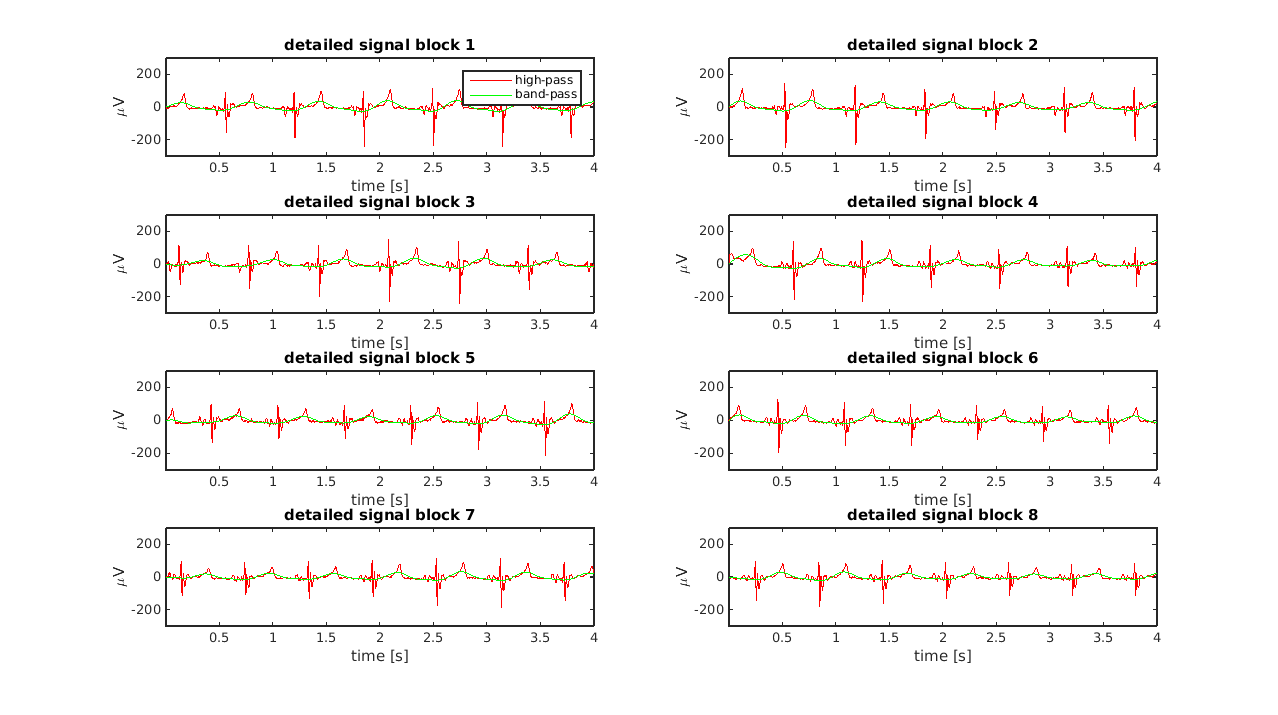
\includegraphics[scale=0.25]{p2fig7.png}
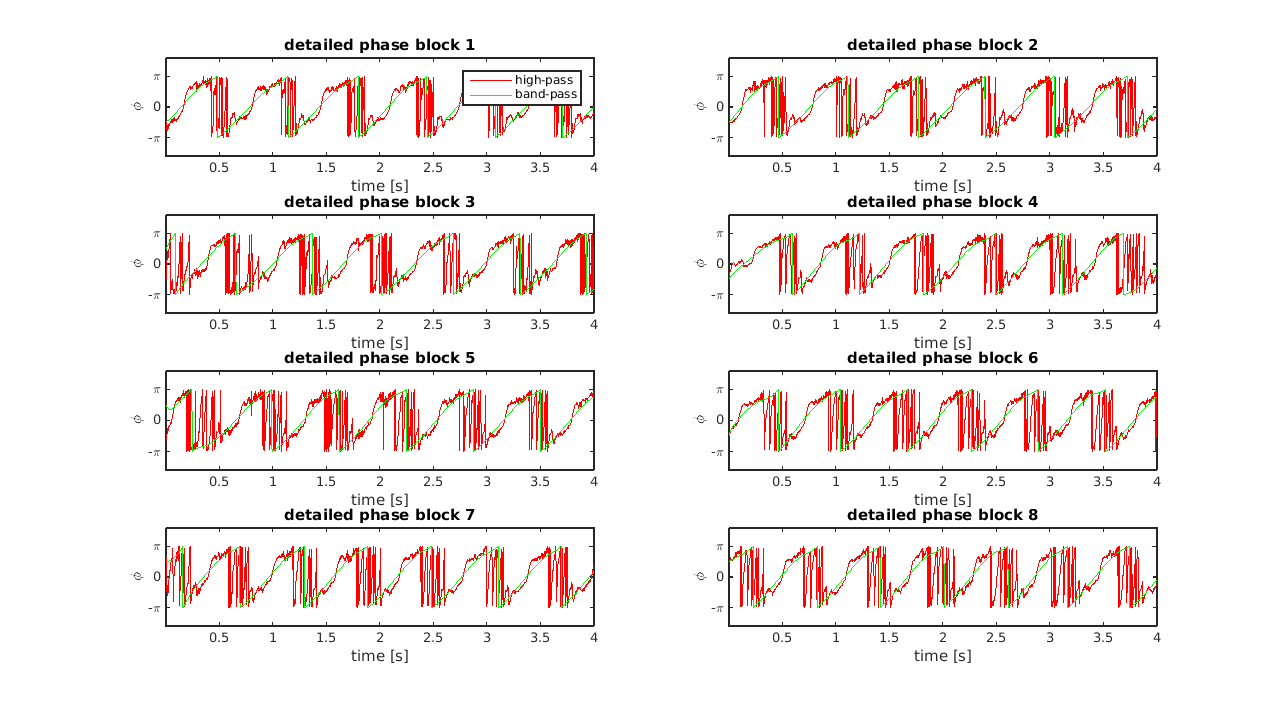
\includegraphics[scale=0.25]{p2fig8.png}

\hspace{-1cm} 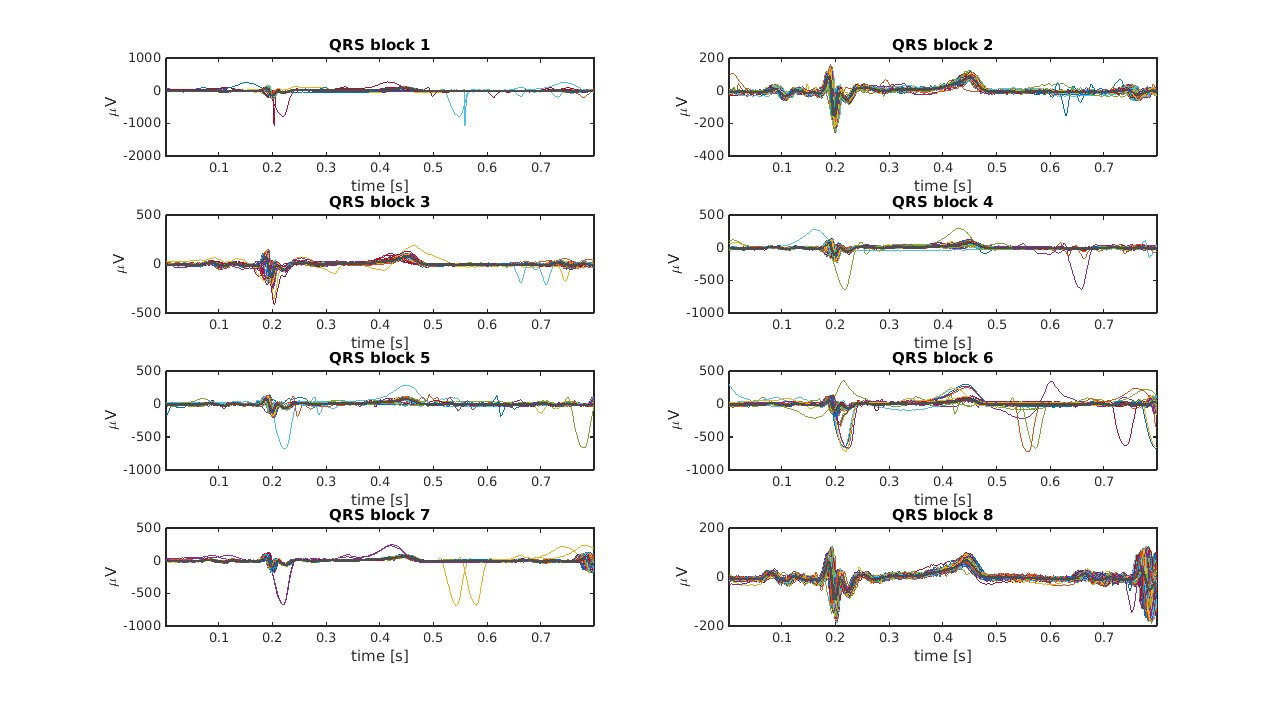
\includegraphics[scale=0.25]{p2fig9.png}
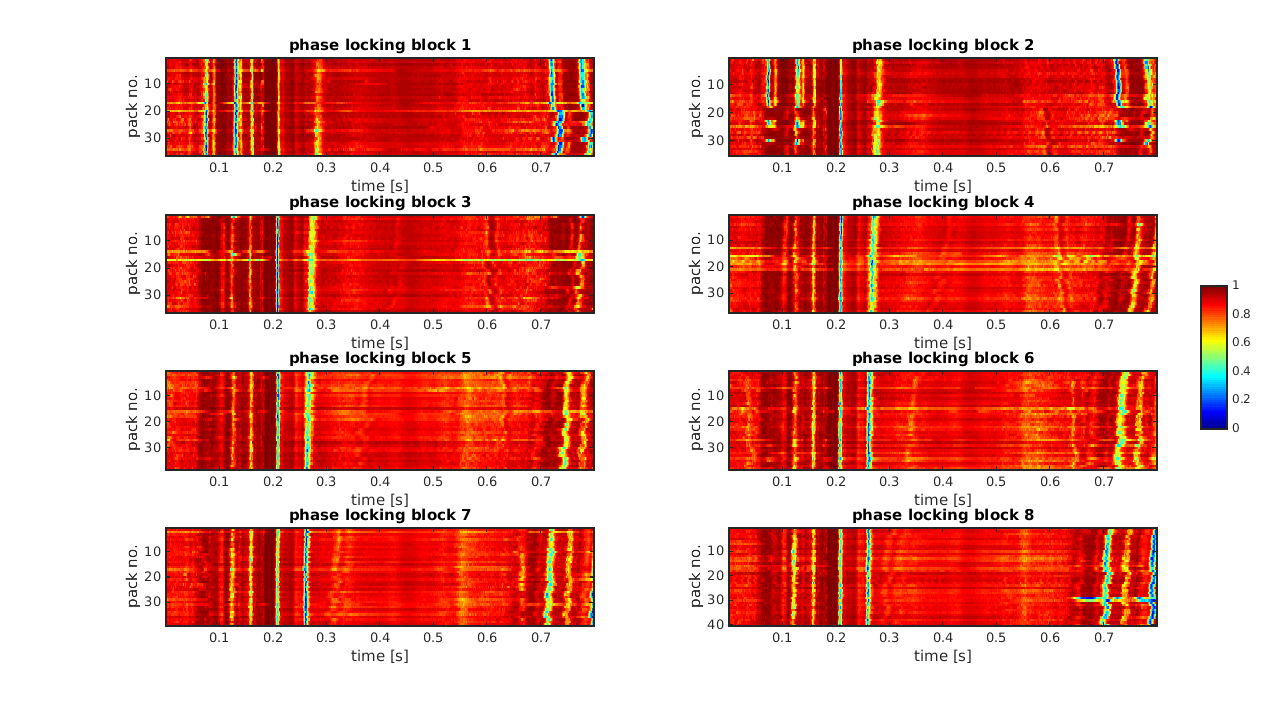
\includegraphics[scale=0.25]{p2fig10.png}
\vspace{5mm}

Compare the signal, phase, and PLV between the 8 levels of blood dilution. Try to identify differences and commonalities between blocks along the epoch. You should leave these figures open when working on the final script.


\section*{Part 3: Classification}
In the last part, we want to process 2 out of the 8 blocks of ECG signals and train 3 binary classifiers on the data: the logit model, and a soft-margin SVM with either a linear kernel or an RBF (aka Gaussian) kernel.

\texttt{runECG3.m} starts as before, in addition specifying the 2 blocks of choice and initializing a variable to store the features.

\begin{minted}[xleftmargin=1cm]{matlab}
srate = 512;

load('filterHP_0.5_1.5.mat')
load('filterLP_3_10.mat')

packSize = 11;
useBlocks = [2 7];
Features = struct('PhaseHP', [], 'PhaseBP', [], 'PLVHP', []);

for B=1:2
\end{minted}

Apparently, we're going to compute phases for the high-pass and band-pass filtered signal and phase locking for the high-pass filtered signal. Fill the gaps in the remainder of the analysis section of the code. This is almost identical to the previous script. In the end, we have a variable \texttt{Features} containing the 3 feature matrices for each of the two blocks, excluding the $2m$ ill-defined epochs.

\begin{minted}[xleftmargin=1cm]{matlab}
load(['block_' num2str(useBlocks(B))])
signal = block_data(:, 3);

...

Features(B).PhaseHP = phasesHP(:, margin+1:end-margin);
Features(B).PhaseBP = phasesBP(:, margin+1:end-margin);
Features(B).PLVHP = plvHP(:, margin+1:end-margin);
\end{minted}

Now we want to train and validate a model on these features. Specifically, we want to specify 2 time points at which we "sample" from each of the 3 features for each epoch.

\begin{minted}[xleftmargin=1cm]{matlab}
t1 = ...
t2 = ...
\end{minted}

From your previous analyses and Scheller et al., 2011, derive 2 time points that correspond roughly to the QRS peak and the T wave of the typical epoch. Note that we have set all phases to zero exactly at the QRS peak, so \texttt{t1} has to be a point shortly before or after the actual peak.

We can now construct the feature matrix by iterating over the two blocks and putting the 6 feature values for each epoch in the corresponding row of \texttt{X}. For simplicity, we use the same number of epochs \texttt{nEpochs} from both blocks, in case they differ in length.

\begin{minted}[xleftmargin=1cm]{matlab}
nEpochs = min(size(Features(1).PhaseHP, 2), size(Features(2).PhaseHP, 2));
X = nan(2*nEpochs, 6);
for B=1:2
    rows = (B-1)*nEpochs + (1:nEpochs);
    X(rows, 1) = ...
    X(rows, 2) = ...
    ...
end
\end{minted}

Finally, we train different models on the data.

\begin{minted}[xleftmargin=1cm]{matlab}
kCross = 10;
L = [ones(nEpochs, 1); zeros(nEpochs, 1)];
modelType = {'logreg', 'linsvm', 'rbfsvm'};
for iModel=1:3
    pCorrect = modelFitVal2(X, L, kCross, modelType{iModel});
    fprintf('\nPerformance %6s: %3i %%\n', modelType{iModel}, round(100*pCorrect));
end
\end{minted}

There is nothing to edit here, but we have to extend our function \texttt{modelFitVal.m} such that it takes an additional input string to specify the model to use (\texttt{'logreg'}, \texttt{'linsvm'}, or \texttt{'rbfsvm'}) and implements the different training and validation procedures accordingly. Fill the missing parts in \texttt{modelFitVal2.m} to implement the 3 different cases. Find the appropriate functions to train SVMs in the MATLAB documentation.

\begin{minted}[xleftmargin=1cm]{matlab}
...

if strcmp(modelType, 'logreg')
    coeff = glmfit(xTrain, lTrain, 'binomial', 'link', 'logit');
    lPredicted = round(glmval(coeff, xTest, 'logit'));
elseif strcmp(modelType, 'linsvm')
    ...
elseif strcmp(modelType, 'rbfsvm')
    ...
else
    error('Unknown model type.');
end

pCorrect = pCorrect + 1/k*mean(lPredicted==lTest);

...
\end{minted}

Each case should produce a variable \texttt{lPredicted} containing the vector of predicted labels per partition.

Once you're done, \texttt{runECG3.m} should print the cross-validated performance of each model, which should ideally be above 90 \%. If not, try to improve performance by varying \texttt{t1} and \texttt{t2}, or check your signal processing steps. If one or more of your models perform at around 50 \%, something is seriously wrong. The same probably goes for exactly 100 \%. Otherwise, you solved the problem.

\end{document}
